Dieses Experiment zeigt eine beispielhafte Situation, in dieser der CoDy Algorithmus mit anderen Ablauf-Varianten schlechter funktionieren würde als mit dem verketteten Ablauf. Für den parallelen Ablauf, zum Beispiel, wäre es erforderlich, dass die Agenten ihre Prioritäten anpassen um einen der beiden Engstellen für sich zu beanspruchen. 

\textbf{Aufbau des Experiments}
\begin{figure}[H]
    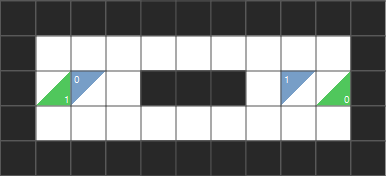
\includegraphics[height=40mm]{images/two_slits.png}
    \centering
    \caption{Aufbau für ein Szenario in dem sich zwei Agenten zwischen zwei Wegen entscheiden}
    \label{fig:doppelspalt}
\end{figure}
Auch hier misst die Karte neun mal drei Felder. In der Mitte befinden sich zwei Engstellen die jeweils drei Felder lang und ein Feld breit sind. Für beide Agenten gilt, dass der Weg zu ihren Zielen durch beide Engestellen gleich lang ist.

\textbf{Erwartete Beobachtungen}\newline
Der Agent der zuerst seinen Weg plant reserviert eine der beiden Engstellen für sich. Der zweite Agent plant dann mit der Engstelle die noch frei ist. Wegen der "'Rechts vor Links"' Regel wird Agent 0 immer die südliche Engstelle befahren und Agent 1 die nördliche. Beide Agenten werden im Laufe des Experiment ihre Prioritäten nicht erhöhen.